% =====================================================================
%  MAT257 — Analysis on Manifolds
%  Note-Taking Template, organized by "Day"
%  --------------------------------------------------------------------
%  Soft, muted accent colors (not saturated blocks): Definition (blue),
%  Theorem (amber/yellow), Example (green). Everything else (Lemma,
%  Proposition, Corollary, Remark, Proof) is now PLAIN TEXT — bold
%  title only, no box / frame / background.
% =====================================================================

\documentclass[11pt]{article}

% ---------- Page & Fonts ----------
\usepackage[margin=1in]{geometry}
\usepackage[utf8]{inputenc}
\usepackage[T1]{fontenc}
% \usepackage{lmodern}      % enable on Overleaf / full TeX installs
% \usepackage{mathpazo}     % nicer serif math font; enable if available
% \usepackage{microtype}    % enable if available — nicer justification

% ---------- Math ----------
\usepackage{amsmath, amssymb, amsfonts}
\usepackage{amsthm}
\usepackage{mathtools}
\usepackage{bm}

% ---------- Colors & Boxes ----------
\usepackage[most]{tcolorbox}
\usepackage{xcolor}

% ---------- Misc ----------
\usepackage{enumitem}
\usepackage{hyperref}
\usepackage{titlesec}
\usepackage{fancyhdr}
\usepackage{tikz}
\usepackage{framed}
\usepackage{etoolbox}
\usetikzlibrary{arrows.meta}

% ---------- Color palette (soft / muted) ----------
\definecolor{defColor}{HTML}{5B8DEF}    % soft blue   - Definition
\definecolor{thmColor}{HTML}{E0A030}    % soft amber/yellow - Theorem
\definecolor{exColor}{HTML}{4CA37A}     % soft green  - Example
\definecolor{neutralColor}{HTML}{8B8F98}% soft gray   - used only for text accents now
\definecolor{inkColor}{HTML}{2D3138}    % near-black text

% ---------- The 3 "headline" boxes — soft tinted style, no solid blocks ----------
\newtcbtheorem[number within=section]{definition}{Definition}%
{colback=defColor!5, colframe=defColor!65, fonttitle=\bfseries,
 coltitle=defColor!75!black, colbacktitle=defColor!12,
 boxrule=0.6pt, arc=1.5mm,
 left=6pt, right=6pt, top=4pt, bottom=4pt,
 breakable, enhanced jigsaw}{def}

\newtcbtheorem[use counter from=definition]{theorem}{Theorem}%
{colback=thmColor!6, colframe=thmColor!70, fonttitle=\bfseries,
 coltitle=thmColor!60!black, colbacktitle=thmColor!15,
 boxrule=0.6pt, arc=1.5mm,
 left=6pt, right=6pt, top=4pt, bottom=4pt,
 breakable, enhanced jigsaw}{thm}

\newtcbtheorem[use counter from=definition]{example}{Example}%
{colback=exColor!5, colframe=exColor!65, fonttitle=\bfseries,
 coltitle=exColor!70!black, colbacktitle=exColor!12,
 boxrule=0.6pt, arc=1.5mm,
 left=6pt, right=6pt, top=4pt, bottom=4pt,
 breakable, enhanced jigsaw}{ex}

% =====================================================================
% ---------- Everything else: PLAIN (no fill, no frame) but with a
%  quiet vertical rule + generous spacing, so items stay easy to tell
%  apart and don't run into each other on the page.
% =====================================================================

% -- generous, well-separated spacing for the "plain" theorem-likes --
\newtheoremstyle{quiet}%
  {12pt}{12pt}%          space above / below
  {\normalfont}{0pt}%    body font / indent
  {\bfseries}{.}%        head font / punctuation after head
  {0.6em}{}%             space after head / custom head-spec
\theoremstyle{quiet}

\newtheorem{proposition}{Proposition}
\newtheorem{lemma}{Lemma}
\newtheorem{corollary}{Corollary}

\makeatletter
\let\c@proposition\c@definition
\let\c@lemma\c@definition
\let\c@corollary\c@definition
\makeatother

\renewcommand{\theproposition}{\thedefinition}
\renewcommand{\thelemma}{\thedefinition}
\renewcommand{\thecorollary}{\thedefinition}

\newtheoremstyle{quietremark}%
  {12pt}{12pt}%
  {\normalfont\itshape}{0pt}%
  {\bfseries\itshape}{.}%
  {0.6em}{}
\theoremstyle{quietremark}
\newtheorem{remark}{Remark}[section]

% -- the quiet left-rule "bar" that visually separates a statement
%    from surrounding prose without drawing a full box --
\definecolor{barColor}{HTML}{8B8F98}
\newenvironment{quietbar}{%
  \def\FrameCommand{{\color{barColor!55}\vrule width 1.1pt\hspace{9pt}}}%
  \MakeFramed{\advance\hsize-\width\relax \FrameRestore}%
}{%
  \endMakeFramed
}
% Auto-wrap every plain theorem-like statement in the quiet bar.
\BeforeBeginEnvironment{lemma}{\begin{quietbar}}
\AfterEndEnvironment{lemma}{\end{quietbar}}
\BeforeBeginEnvironment{proposition}{\begin{quietbar}}
\AfterEndEnvironment{proposition}{\end{quietbar}}
\BeforeBeginEnvironment{corollary}{\begin{quietbar}}
\AfterEndEnvironment{corollary}{\end{quietbar}}
\BeforeBeginEnvironment{remark}{\begin{quietbar}}
\AfterEndEnvironment{remark}{\end{quietbar}}

% Proof: same quiet left-rule treatment, ending in a small solid QED square.
\providecommand{\qedsymbol}{$\blacksquare$}
\newenvironment{myproof}{%
  \begin{quietbar}\par\vspace{2pt}\noindent\textbf{Proof.}\ %
}{%
  \hfill\qedsymbol\par\vspace{2pt}\end{quietbar}\vspace{6pt}%
}

% ---------- Section styling ----------
\titleformat{\section}
 {\normalfont\Large\bfseries\color{inkColor}}
 {\thesection}{0.6em}{}
 [{\color{neutralColor!35}\titlerule[0.8pt]}]
\titleformat{\subsection}
 {\normalfont\large\bfseries\color{inkColor}}
 {\thesubsection}{0.6em}{}

% ---------- Hyperref colors ----------
\hypersetup{
 colorlinks=true,
 linkcolor=inkColor,
 citecolor=exColor,
 urlcolor=defColor,
 pdftitle={MAT257 Notes},
 pdfauthor={}
}

% ---------- Quick math macros (common in analysis courses) ----------
\newcommand{\R}{\mathbb{R}}
\newcommand{\N}{\mathbb{N}}
\newcommand{\Z}{\mathbb{Z}}
\newcommand{\Q}{\mathbb{Q}}
\newcommand{\C}{\mathbb{C}}
\newcommand{\eps}{\varepsilon}
\newcommand{\norm}[1]{\left\lVert #1 \right\rVert}
\newcommand{\abs}[1]{\left\lvert #1 \right\rvert}
\newcommand{\dd}{\mathrm{d}}
\DeclareMathOperator{\rank}{rank}
\DeclareMathOperator{\Int}{int}   % interior of a set, e.g. \Int(A)

% =====================================================================
% ---------------------------- COVER PAGE ------------------------------
% =====================================================================
\begin{document}

\begin{titlepage}
\centering
\vspace*{1.3cm}

{\Large\textsc{Lecture Notes}}\\[0.4cm]
{\color{neutralColor!50}\rule{0.35\textwidth}{0.6pt}}\\[1.0cm]

{\fontsize{32}{38}\selectfont\bfseries MAT257}\\[0.3cm]
{\Large\itshape Analysis on Manifolds}\\[1.0cm]

% ---------------- Manifold illustration ----------------
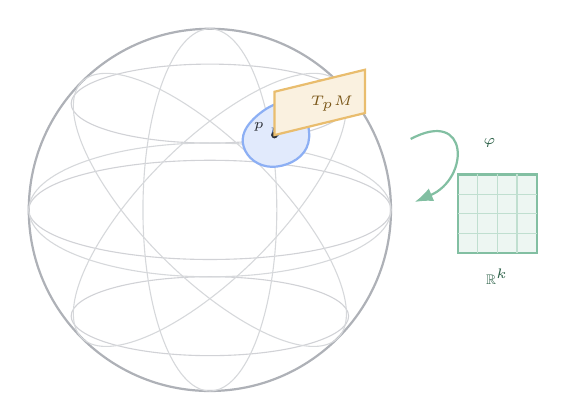
\begin{tikzpicture}[scale=1.0]
  % --- sphere-like manifold, drawn with a grid of "meridians" and "parallels" ---
  \begin{scope}
    % outer silhouette
    \draw[neutralColor!70, thick] (0,0) circle (2.3cm);
    % parallels (horizontal ellipses), thinning toward the poles
    \foreach \h/\o in {1.35/40, 0/0, -1.35/40}{
      \draw[neutralColor!40, thin]
        (0,\h) ellipse ({2.3*cos(\o)} and {0.55*cos(\o)+0.08});
    }
    % meridians: 4 evenly-spaced great circles (0 and 180 coincide, so skip 180)
    \foreach \a in {0,45,90,135}{
      \draw[neutralColor!35, thin, rotate=\a] (0,0) ellipse (0.85 and 2.3);
    }
  \end{scope}

  % --- highlighted coordinate chart patch U on the surface ---
  \draw[defColor!70, fill=defColor!18, thick]
     plot [smooth cycle, tension=0.8]
     coordinates {(0.55,1.15) (1.05,1.35) (1.25,0.85) (0.85,0.55) (0.45,0.75)};
  \node[defColor!70!black, font=\tiny] at (0.85,0.98) {$U$};

  % --- point p on the patch, tangent plane, and normal-ish accent ---
  \fill[inkColor] (0.82,0.95) circle (1.2pt);
  \node[inkColor, font=\tiny] at (0.62,1.05) {$p$};

  % tangent plane as a small parallelogram touching at p, in amber accent
  \draw[thmColor!70, fill=thmColor!15, thick]
     (0.82,0.95) -- ++(1.15,0.28) -- ++(0.0,0.55) -- ++(-1.15,-0.28) -- cycle;
  \node[thmColor!55!black, font=\tiny] at (1.55,1.35) {$T_pM$};

  % --- arrow to a small coordinate square, representing the chart map phi ---
  \draw[exColor!70, -Latex, thick] (2.55,0.9) .. controls (3.3,1.3) and (3.3,0.4) .. (2.6,0.1);
  \node[exColor!60!black, font=\tiny] at (3.55,0.85) {$\varphi$};
  \draw[exColor!70, fill=exColor!10, thick] (3.15,-0.55) rectangle (4.15,0.45);
  \foreach \x in {3.4,3.65,3.9}{\draw[exColor!35] (\x,-0.55) -- (\x,0.45);}
  \foreach \y in {-0.3,-0.05,0.2}{\draw[exColor!35] (3.15,\y) -- (4.15,\y);}
  \node[exColor!60!black, font=\tiny] at (3.65,-0.85) {$\R^k$};

\end{tikzpicture}

\vspace{0.3cm}


\vspace{1.4cm}
{\large Fuxuan Xu}\\[0.2cm]
{\large University of Toronto}

\vfill

\begin{tcolorbox}[colback=black!2, colframe=neutralColor!35, width=0.7\textwidth,
 arc=1.5mm, boxrule=0.4pt]
\centering\small
\textbf{How this notebook works}\\[3pt]
Notes are grouped \textbf{by day} (Day 1, Day 2, \dots) rather than by topic,
matching the order things were covered in lecture. Only three box types carry
color --- \textcolor{defColor!75!black}{\textbf{Definition}} (blue),
\textcolor{thmColor!60!black}{\textbf{Theorem}} (amber), and
\textcolor{exColor!70!black}{\textbf{Example}} (green) --- kept soft and light
so they're easy on the eyes. Everything else (Lemma, Proposition, Corollary,
Remark, Proof) is plain text with a bold label, no box.
\end{tcolorbox}

\vspace{1.0cm}
\end{titlepage}

\tableofcontents
\newpage

% =====================================================================
\section{Day 1 (9.9) --- Continuity and Norms}
% =====================================================================
\begin{definition}{Continuity (Tentative)}
\text{A scalar function $f(x_1,\cdots,x_n)$ is continuous if it's continuous on function of each $x_i$. More generally, vector-valued function $f(x_1,\cdots,x_n)$ is continuous if all $f_j(x_1,\cdots,x_n)$ are continuous.}
\end{definition}

\begin{example}{Counterexample}
\text{Consider the function $f(x,y)=\begin{cases}\frac{xy}{x^2+y^2},(x,y)\ne (0,0)\\0,(x,y)=(0,0)\end{cases}$ is not continuous, although it is continuous for both $x$ and $y$.}
\end{example}

\begin{definition}{Limit (Tentative)}
\text{A scalar function $f:\mathbb{R}^n\to\mathbb{R}$ has its limit exist at $(x_1,\cdots,x_n)$ if for every direction vector $(a_1,\cdots,a_n)$, $\lim_{t\to 0}f(x_1+ta_1,\cdots,x_n+ta_n)$ exists and does not depend on $a=(a_1,\cdots,a_n).$}
\end{definition}

\begin{example}{Counterexample}
\text{Consider the function $f(x,y)=\begin{cases}\frac{y}{x^2}. x\ne 0\\0,x=0\end{cases}$. We take the direction $(a_1,a_2)$ such that $a_1\ne 0$, and we plug this into $f$ and we have $f(ta_1,ta_2)=\frac{ta_2}{t^2a_1^2}=\frac{a_2}{ta_1^2}$, and when $t\to 0$, the expression goes to $\pm \infty$, and the limit does not exist. }
\end{example}

\begin{definition}{Continuity (Tentative)}
\text{Let $x=(x_1,\cdots,x_n)\in\mathbb{R}^n$, then $f:\mathbb{R}^n\to\mathbb{R}$ is continuous at $x\in\mathbb{R}^n$ if $\lim_{h\to 0}f(x+h)=f(x)$.}
\end{definition}

To define the term “$\lim$” in $\mathbb{R}^n$, we have to go into the topology of $\mathbb{R}^n$. 

\begin{definition}{Norm}
\text{A norm on a vector space is a function $\|\cdot\|:V\to \mathbb{R}_{\ge 0}$ such that:
\begin{enumerate}
\item $\|v\|=0$ iff $v=0$.
\item $\|tv\|=|t|\|v\|$ for all $t\in\mathbb{R}$ and $v\in V$.
\item Triangle inequality: $\|v+w\|\le\|v\|+\|w\|$ for all $v,w\in V$.
\end{enumerate}}
\end{definition}

Since $\mathbb{R}^n$ is a vector space, we can define the standard norm of $\mathbb{R}^n$, we let $x=(x_1,\cdots,x_n)$ so we have 
\[
\|x\|=\sqrt{x_1^2+\cdots+x_n^2}.
\]
Another important norm of $\mathbb{R}^n$ is the sup-norm:
\[
\|x\|_\infty=\max\{|x_1|,\cdots,|x_n|\}.
\]
% =====================================================================
\newpage

\section{Day 2 (9.11) --- Equivalent Norms, Continuity and Open Sets}
% =====================================================================
Consider the norms:\\
If $\|x\|\le R$, then $x$ is contained in a closed ball with radius $R$. If $\|x\|_\infty\le R$, then $x$ is contained in a closed rectangle $[-R,R]^n$. An example of a norm on an infinite dimensional vector space $C({[a,b]})$ such that $[a,b]\subseteq\mathbb{R}$ is $\|f\|_\infty=\sup\{|f(x)|:x\in[a,b]\}$.

\begin{theorem}{}
\text{Let $x\in\mathbb{R}^n$, then $\|x\|_\infty\le \|x\|\le\sqrt{n}\|x\|_\infty.$ }
\end{theorem}
\begin{proof}
We know that $\|x\|_\infty = \max \{|x_1|, \dots, |x_n|\}$. 
For the lower bound, since each term is non-negative, we have:
\[
\|x\|_\infty^2 = \max_i |x_i|^2 \le \sum_{i=1}^n x_i^2 = \|x\|^2,
\]
which implies $\|x\|_\infty \le \|x\|$.

For the upper bound, summing over all $n$ components gives:
\[
\|x\|^2 = \sum_{i=1}^n x_i^2 \le \sum_{i=1}^n \left(\max_j |x_j|\right)^2 = n \|x\|_\infty^2.
\]
Taking the square root on both sides yields $\|x\| \le \sqrt{n} \|x\|_\infty$.
Thus, $\|x\|_\infty \le \|x\| \le \sqrt{n} \|x\|_\infty$.
\end{proof}
\begin{definition}{Equivalent Norms}
\text{Two norms $\|\cdot\|_1, \|\cdot\|_2$ on vector space $V$ are equivalent if $\exists c,C>0 \text{ s.t. } c\|x\|_1\le\|x\|_2\le C\|x\|_1$.}
\end{definition}

\begin{example}{}
\text{$\|\cdot\|_\infty$ and $\|\cdot\|$ are equivalent norms on $\mathbb{R}^n$ since we can choose $c=1, C=\sqrt{n}$ to make 
\[
\|x\|_\infty \le \|x\| \le \sqrt{n}\|x\|_\infty.
\]}
\end{example}

\begin{lemma}
\text{Any two norms on $\mathbb{R}^n$ are equivalent.}
\end{lemma}

\begin{definition}{Continuous}
\text{A function $f:A\subseteq\mathbb{R}^n\to\mathbb{R}^m$ is continuous at $x_0\in A$ if:
\[
\forall\varepsilon>0,\exists\delta>0, \text{ s.t. }\|x-x_0\|<\delta\Rightarrow \|f(x)-f(x_0)\|<\varepsilon.
\]
$f$ is continuous if it is continuous everywhere.}
\end{definition}

There, we can replace the Euclidean norm $\|\cdot\|$ by any equivalent norm. Also, the subset $A$ is any subset of $\mathbb{R}^n$. Moreover, if $f:A\to\mathbb{R}^n$ is continuous and $A_1\subseteq A$, then $f|_A$ is continuous.

\begin{proposition}{Composition of Continuous Functions is Continuous}
Let $A\subseteq\mathbb{R}^n, B\subseteq\mathbb{R}^m$, and $f,g$ be functions such that $f:A\to\mathbb{R}^m, g:B\to\mathbb{R}^k$ with $f(A)\subseteq B$. If $f$ is continuous at $x_0$ and $g$ is continuous at $f(x_0)$, then $g\circ f:A\to\mathbb{R}^k$ is continuous at $x_0$. In particular, if $f,g$ are continuous, then $g\circ f$ is continuous.
\end{proposition}

\begin{proof}
Let $\varepsilon>0$ be given. Since $g$ is continuous at $f(x_0)$, then $\exists\delta_g>0$ such that:
\[
\|y-f(x_0)\|<\delta_g\Rightarrow\|g(y)-(g\circ f)(x)\|<\varepsilon.
\]
Since $f$ is continuous at $x_0$, then $\exists\delta_f>0$ such that: 
\[
\|x-x_0\|<\delta_f\Rightarrow \|f(x)-f(x_0)\|<\varepsilon.
\]
We take the radius corresponding to  $\delta_g$ for $f$, so that:
\[
\|x-x_0\|<\delta_f\Rightarrow\|f(x)-f(x_0)\|<\delta_g,
\]
and this implies that: 
\[
\|x-x_0\|<\delta_f\Rightarrow\|(g\circ f)(x)-(g\circ f)(x_0)\|<\varepsilon,
\]
as desired.
\end{proof}

\begin{proposition}
The set of continuous functions $f:A\to\mathbb{R}^m$ is a vector space.
\end{proposition}

\begin{proof}
As an exercise.
\end{proof}

\begin{proposition}
A function $f:A\to\mathbb{R}^m$ can be expressed as $f=(f_1,\cdots,f_n)$ for $i\in\{1,\cdots,n\}$, then $f$ is continuous iff all of its component functions $f_i:A\to\mathbb{R}$ are continuous.
\end{proposition}

\begin{proof}
As an exercise. Hint: use the sup-norm $\|f(x)-f(x_0)\|_\infty$.
\end{proof}

\begin{definition}{Open Ball}
\text{The open ball around $x\in\mathbb{R}^n$ is defined as:
\[
B_\varepsilon(x)=\{y\in\mathbb{R}^n\mid\|x-y\|<\varepsilon\}.
\]}
\end{definition}

\begin{definition}{Open Set}
\text{A subset $M\subseteq\mathbb{R}^n$ is an open set if $\forall x\in M, \exists \varepsilon>0 \text{ s.t. } B_\varepsilon(x)\subseteq M$.}
\end{definition}

\begin{definition}{Open Neighborhood}
\text{An open neighborhood of $x\in\mathbb{R}^n$ is an open subset $U$ with $x\in U$.}
\end{definition}

\newpage
% =====================================================================
\section{Day 3 --- }
% =====================================================================

% =====================================================================
\section{Day 4 --- }
% =====================================================================


% =====================================================================
\section{Day 5 --- }
% =====================================================================


% =====================================================================

\section{Day 6 --- }
% =====================================================================


% ====================================================================


\section{Day 7 --- }
% =====================================================================


% ====================================================================


\section{Day 8 --- }
% =====================================================================


% ====================================================================


\section{Day 9 --- }
% =====================================================================


% ====================================================================


\section{Day 10 --- }
% =====================================================================


% ====================================================================


\section{Day 11 --- }
% =====================================================================


% ====================================================================


\section{Day 12 --- }
% =====================================================================


% ====================================================================


\section{Day 13 --- }
% =====================================================================


% ====================================================================


\section{Day 14 --- }
% =====================================================================


% ====================================================================


\section{Day 15 --- }
% =====================================================================


% ====================================================================


\section{Day 16 --- }
% =====================================================================


% ====================================================================


\section{Day 17 --- }
% =====================================================================


% ====================================================================


\section{Day 18 --- }
% =====================================================================


% ====================================================================
\section*{Notes \& Questions}
\addcontentsline{toc}{section}{Notes \& Questions}
% =====================================================================

\begin{tcolorbox}[colback=black!2, colframe=neutralColor!40, arc=1.5mm, breakable]
\begin{itemize}[leftmargin=*]
  \item[$\square$] Review the proof of the Inverse Function Theorem in detail.
  \item[$\square$] Redo the change-of-variables example from lecture with polar coordinates.
  \item[$\square$] Ask TA: why does $Dh$ need full rank in the manifold definition?
\end{itemize}
\end{tcolorbox}

\end{document}
